\chapter{Projective Varieties (In Progress)}
Having studied affine varieties in $\Aff^n$, we now consider $\CP^n$.
We will also make it into a baby ringed space
in the same way as with $\Aff^n$.

\section{Graded Rings}
\prototype{$\CC[x_0, \dots, x_n]$ is a graded ring.}
We first take the time to state what a graded ring is,
just so that we have this language to use (now and later).

\begin{definition}
	A \vocab{graded ring} $R$ is a ring with the following additional structure:
	as an abelian group, it decomposes as
	\[ R = \bigoplus_{d \ge 0} R^d \]
	where $R^0$, $R^1$, \dots, are abelian groups.
	The ring multiplication is required to satisfy the following property:
	if $r \in R^d$ and $s \in R^e$, we have $rs \in R^{d+e}$.
	Elements of an $R^d$ are called \vocab{homogeneous elements}.

	We denote by $R^+$ the ideal $R \setminus R_0$ generated by
	the homogeneous elements of nonzero degree,
	and call it the \vocab{irrelevant ideal}.
\end{definition}
\begin{remark}
	For algebraic geometry,
	our graded rings will always have unit and be commutative.
\end{remark}
\begin{example}
	[Examples of Graded Rings]
	\listhack
	\begin{enumerate}[(a)]
		\ii The ring $\CC[x]$ is graded by degree.
		\ii More generally, the polynomial ring $\CC[x_0, \dots, x_n]$
		is graded by degree.
	\end{enumerate}
\end{example}

We will frequently refer to homogeneous ideals:
\begin{definition}
	An ideal $I \subseteq \CC[x_0, \dots, x_n]$ is \vocab{homogeneous}
	if it can be written as $I = (f_1, \dots, f_m)$
	where each $f_i$ is a homogeneous polynomial.
\end{definition}
\begin{remark}
	If $I$ and $J$ are homogeneous,
	then $I+J$, $I \cap J$, $\sqrt I$ are homogeneous too.
\end{remark}
\begin{lemma}[Graded Quotients are Graded Too]
	Let $I$ be a homogeneous ideal of a graded ring $R$.
	Then
	\[ R/I = \bigoplus_{d \ge 0} R_d / (R_d \cap I) \]
	realizes $R/I$ as a graded ring.
\end{lemma}
Since these assertions are just algebra,
we omit their proofs here.
\begin{example}
	[Example of a Graded Quotient Ring]
	Let $R = \CC[x,y]$ and set $I = (x^3, y^2)$. Then
	\begin{align*}
		R^0 &= \CC \\
		R^1 &= \CC x \oplus \CC y \\
		R^2 &= \CC x^2 \oplus \CC xy \\
		R^3 &= \CC x^2y \\
		R^d &= 0 \qquad \forall d \ge 4.
	\end{align*}
	So in fact $R/I$ is graded, and is a six-dimensional $\CC$-vector space.
\end{example}


\section{The Ambient Space}
\prototype{Perhaps $\VV(x^2+y^2-z^2)$ work.}
The set of points we choose to work with is $\CP^n$ this time,
which for us can be thought of as the set of $n$-tuples
\[ \left( x_0 : x_1 : \dots : x_n \right) \]
not all zero, up to scaling.
Equivalently, it is the set of lines through the origin in $\CC^{n+1}$.
Projective space is defined in full in \Cref{sec:top_spaces},
and you should refer there if you aren't familiar with projective space.

The right way to think about it is ``$\Aff^n$ plus points at infinity'':
\begin{definition}
	We define the set
	\[ U_i = \left\{ (x_0 : \dots : x_n) \mid x_i \neq 0  \right\}
		\subseteq \CP^n. \]
	These are called the \vocab{standard affine charts}.
\end{definition}
The name comes from the following:
\begin{exercise}
	(Mandatory)
	Give a natural bijection from $U_i$ to $\Aff^n$.
	Thus we can think of $\CP^n$ as the affine set $U_i$
	plus ``points at infinity''.
\end{exercise}
\begin{remark}
	In fact, these charts $U_i$ make $\CP^n$ with its usual topology
	into a complex manifold with holomorphic transition functions.
\end{remark}

However, like before we want to impose a Zariski topology on it.
For concreteness, let's consider $\CP^2 = \left\{ (x_0 : x_1 : x_2) \right\}$.
We wish to consider zero loci in $\CP^2$, just like we did in affine space,
and hence obtain a notion of a projective variety.

But this isn't so easy: for example,
the function ``$x_0$'' is not a well-defined function on points in $\CP^2$ 
because $(x_0 : x_1 : x_2) = (5x_0 : 5x_1 : 5x_2)$!
So we'd love to consider these ``pseudo-functions''
that still have zero loci. These are just the homogeneous polynomials $f$,
because $f$ is homogeneous of degree $d$ if and only if
\[
	f(\lambda x_0, \dots, \lambda x_n)
	= \lambda^d f(x_0, \dots, x_n).
\]
In particular, the relation ``$f(x_0, \dots, x_n) = 0$'' is
well-defined if $F$ is homogeneous. Thus, we can say:
\begin{definition}
	If $f$ is homogeneous, we can then define its \vocab{vanishing locus} as
	\[
		\VV(f)
		= \left\{ (x_0 : \dots : x_n) \mid f(x_0, \dots, x_n) = 0 \right\}.
	\]
\end{definition}

The homogeneous condition is really necessary.
For example, to require ``$x_0 - 1 = 0$'' makes no sense,
since the points $(1:1:1)$ and $(2015:2015:2015)$ are the same.

It's trivial to verify that homogeneous polynomials do exactly what we want:
hence we can do the following.
\begin{definition}
	A \vocab{projective variety} in $\CP^n$
	is the common zero locus of an arbitrary
	collection of homogeneous polynomials in $n+1$ variables.
\end{definition}

\begin{example}[A Conic in $\CP^2$, or a Cone in $\CC^3$]
	Let's try to picture the variety
	\[ \VV(x^2+y^2-z^2) \subseteq \CP^2 \]
	which consists of the points $[x:y:z]$ such that $x^2+y^2=z^2$.
	If we view this as subspace of $\CC^3$
	(i.e.\ by thinking of $\CP^2$ as the set of lines through the origin),
	then we get a ``cone'':
	\begin{center}
		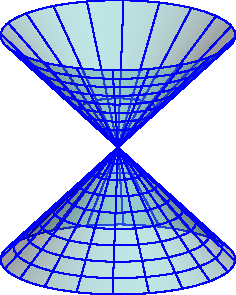
\includegraphics{media/cone.pdf}
	\end{center}

	If we take the standard affine charts now, we obtain the following:
	\begin{itemize}
		\ii At $x=1$, we get a hyperbola $\VV(1+y^2-z^2)$.
		\ii At $y=1$, we get a hyperbola $\VV(1+x^2-z^2)$.
		\ii At $z=1$, we get a circle $\VV(x^2+y^2-1)$.
	\end{itemize}
	That said, over $\CC$ a hyperbola and circle
	are the same thing; I'm cheating a little by drawing $\CC$
	as one-dimensional, just like last chapter.
\end{example}
\begin{ques}
	Draw the intersection of the cone above
	with the $z=1$ plane, and check that you do in fact get a circle.
	(This geometric picture will be crucial later.)
\end{ques}

\section{Homogeneous Ideals}
Now, the next thing we want to do is define $\VV(I)$ for an ideal $I$.
Of course, we again run into an issue with things like $x_0-1$ not
making sense. 

The way out of this is to use only \emph{homogeneous} ideals.
\begin{definition}
	If $I$ is a homogeneous ideal, we define
	\[ \VV(I) = \{ x \mid f(x) = 0 \; \forall f \in I\}. \]
\end{definition}
\begin{exercise}
	Show that the notion ``$f(x) = 0 \; \forall f \in I$''
	is well-defined for a homogeneous ideal $I$.
\end{exercise}
So, we would hope for a nullstellensatz-like theorem
which bijects the homogeneous semiprime ideals to the ideals.
Unfortunately:
\begin{example}
	[Irrelevant Ideal]
	To crush some dreams and hopes, consider the ideal
	\[ I = (x_0, x_1, \dots, x_n). \]
	This is called the \vocab{irrelevant ideal};
	it is homogeneous semiprime
	and has the property that $\VV(I) = \varnothing$.
\end{example}

However, other than the irrelavant ideal.
\begin{theorem}
	[Homogeneous Nullstellensatz]
	Let $I$ and $J$ be homogeneous ideals. 
	\begin{enumerate}[(a)]
		\ii If $\VV(I) = \VV(J) \neq \varnothing$ then $\sqrt I = \sqrt J$.
		\ii If $\VV(I) = \varnothing$, then either $I = (1)$
		or $\sqrt I = (x_0, x_1, \dots, x_n)$.
	\end{enumerate}
	Thus there is a natural bijection between:
	\begin{itemize}
		\ii projective varieties in $\CP^n$, and
		\ii homogeneous semiprime ideas of $\CC[x_1, \dots, x_n]$ 
		except for the irrelevant ideal. 
	\end{itemize}
\end{theorem}
\begin{proof}
	For the first part, let $V = \VV(I)$ and $W = \VV(J)$
	be projective varieties in $\CP^n$.
	We can consider them as \emph{affine varieties} in $\Aff^{n+1}$
	by using the interpretation of $\CP^n$
	as lines through the origin in $\CC^n$.

	Algebraically, this is done by taking the homogeneous ideals
	$I, J \subseteq \CC[x_0, \dots, x_n]$
	and using the same ideals to cut out \emph{affine} varieties
	$V_{\text{aff}} = \VV(I)$ and $W_{\text{aff}} = \VV(J)$ in $\Aff^{n+1}$.
	For example, the cone $x^2+y^2-z^2=0$ is a conic in $\CP^2$,
	but can also be thought of as the two-dimensional cone in $\Aff^3$.

	Then for (a), we have $V_{\text{aff}} = W_{\text{aff}}$,
	so $\sqrt I = \sqrt J$.

	For (b), either $V_{\text{aff}}$ is empty 
	or it is just the origin of $\Aff^{n+1}$,
	so the Nullstellensatz implies either $I = (1)$
	or $\sqrt I = (x_0, \dots, x_n)$ as desired.
\end{proof}


\section{As Ringed Spaces}
\prototype{The regular functions on $\CP^1$ minus a point
are exactly those of the form $P(s/t)$.}
Now, let us make every projective variety $V$ into a baby ringed space.
We already have the set of points, a subset of $\CP^n$.

The topology is defined as follows.
\begin{definition}
	We endow $\CP^n$ with the \vocab{Zariski topology}
	by declaring the sets of the form $\VV(I)$,
	where $I$ is a homogeneous ideal, to be the closed sets.
	
	Every projective variety $V$ then inherits the Zariski
	topology from its parent $\CP^n$.
	The \vocab{distinguished open sets} $D(f)$ are $V \setminus \VV(f)$.
\end{definition}

Thus every projective variety $V$ is now a topological space.
It remains to endow it with a sheaf of regular functions $\OO_V$.
To do this we had to be a little careful.
In the affine case we had a nice little ring of functions,
the coordinate ring $\CC[x_0,\dots,x_n] / I$,
that we could use to provide the numerator and denominators.
So, it seems natural to then define the following:
\begin{definition}
	The \vocab{homogeneous coordinate ring} of a projective variety
	$V = \VV(I) \subseteq \CP^n$, where $I$ is homogeneous semiprime,
	is defined as the ring
	\[ \CC[V] = \CC[x_0, \dots, x_n] / I. \]
\end{definition}
However, when we define rational function we must impose
a new requirement that the numerator and denominator are the same degree.
\begin{definition}
	Let $U \subseteq V$ be an open set of a projective variety $V$.
	A \vocab{rational function} $\phi$ on a projective variety $V$
	is a quotient $f/g$, where $f,g \in \CC[V]$,
	and $f$ and $g$ are homogeneous of the same degree,
	and $\VV(g) \cap U = \varnothing$.
	In this way we obtain a function $\phi : U \to \CC$.
\end{definition}
\begin{example}
	[Examples of Rational Functions]
	Let $V = \CP^1$ have coordinates $(s:t)$.
	\begin{enumerate}[(a)]
		\ii If $U = V$, then constant functions $c/1$
		are the only rational functions on $U$.
		\ii Now let $U_1 = V \setminus \{(1:0)\}$.
		Then, an example of a regular function is
		\[ \frac{s^2+9t^2}{t^2} = \left( \frac st \right)^2 + 9. \]
		If we think of $U_1$ as $\CC$
		(i.e.\ $\CP^1$ minus an infinity point, hence like $\Aff^1$)
		then really this is just the function $x^2+9$.
	\end{enumerate}
\end{example}
Then we can repeat the same definition as before:
\begin{definition}
	Let $U \subseteq V$ be an open set of a projective variety $V$.
	We say a function $\phi : U \to \CC$ is a \vocab{regular function} if
	for every point $p$, we can find an open set $U_p$ containing $p$
	and a rational function $f_p/g_p$ on $U_p$ such that
	\[ \phi(x) = \frac{f_p(x)}{g_p(x)} \qquad \forall x \in U_p. \]
	In particular, we require $U_p \cap \VV(g_p) = \varnothing$.
	We denote the set of all regular functions on $U$ by $\OO_V(U)$.
\end{definition}
Of course, the rational functions from the previous example
are examples of regular functions as well.
This completes the definition of a projective variety $V$
as a baby ringed space.

\section{Examples of Regular Functions}
Naturally, I ought to tell you what the regular functions
on distinguished open sets are; this is an analog to
\Cref{thm:reg_func_distinguish_open} from last time.
\begin{theorem}
	[Regular Functions on Distinguished Open Sets for Projective Varieties]
	Let $V$ be a variety, and let $g \in \CC[V]$ be homogeneous
	of positive degree.
	Then
	\[
		\OO_V(D(g))
		= \left\{ \frac{f}{g^r} \mid
		f \in \CC[V] \text{ homogeneous of degree $r\deg g$}
		\right\}.
	\]
\end{theorem}
What about the case $g = 1$?
A similar result holds, but we need the assumption that $V$ is irreducible.
(This has the same definition as the affine case,
since ``irreducible'' is an adjective of topological spaces.)
\begin{theorem}
	[Only Constant Regular Functions on Projective Space]
	Let $V$ be an \emph{irreducible} projective variety.
	Then the only regular functions on $V$ are constant,
	thus we have \[ \OO_V(V) \cong \CC. \]
\end{theorem}
Proofs of these are omitted for now.
\begin{example}
	[Regular Functions on $\CP^1$]
	Let $V = \CP^1$, with coordinates $(s:t)$.
	\begin{enumerate}[(a)]
		\ii By theorem, if $U_1$ is the standard affine chart
		omitting the point $(1:0)$, we have
		$ \OO_V(U_1) = \left\{ \frac{f}{t^n} \mid \deg f = n \right\} $.
		One can write this as
		\[ \OO_V(U_1) \cong \left\{ P(s/t) \mid P \in \CC[x] \right\}
			\cong \OO_{\Aff^1} (\Aff^1). \]
		This conforms with our knowledge that $U_1$
		``looks very much like $\Aff^1$''.
		\ii As $V$ is irreducible, $\OO_V(V) = \CC$:
		there are no nonconstant functions on $\CP^1$.
	\end{enumerate}
\end{example}

\begin{example}
	[Regular Functions on $\CP^2$]
	Let $\CP^2$ have coordinates $(x:y:z)$ and 
	let $U_0 = \left\{ (x:y:1) \in \CP^2 \right\}$
	be the distinguished open set $D(z)$.
	Then in the same vein,
	\[
		\OO_{\CP^2}(U_0)
		= \left\{ \frac{P(x,y)}{z^n} \mid \deg P = n \right\}
		\cong \left\{ P(x/z, y/z) \mid P \in \CC[x,y] \right\}.
	\]
\end{example}

\section\problemhead
affine and irreducible projective variety not isomorphic unless point


chapter{Bonus: B\'ezout's Theorem}
In this chapter we discuss B\'ezout's Theorem.
It makes precise the idea that two degree $d$ and $e$
curves in $\CP^2$ should intersect at ``exactly'' $de$ points
In order to make this vision come true:
\begin{itemize}
	\ii We ought to work in $\CP^n$,
	so that for example any two lines intersect.
	\ii We need to account for multiplicities.
	So we will whenever possible work with homogeneous ideals $I$,
	because we want to allow the possibility that $I$ is not semiprime.
\end{itemize}

\section{The Hilbert Function}
Let $I \subseteq \CC[x_0, \dots, x_n]$ be homogeneous.


